\documentclass{beamer}
\graphicspath{ {graphics/}}
\begin{document}
\title{Literary Worlds Javascript Client}
\author{John Lewis, Owen Watson, Tim Cunningham}
\usenavigationsymbolstemplate{}
\frame{\titlepage}
\frame{\frametitle{Table of contents}\tableofcontents}

\section{Background}
\frame{\frametitle{Background} 
\begin{itemize}
\item Literary Worlds is an multiuser text based game used for English education at WMU.
\item Most of these text based games provide a telnet interface for playing, Literary Worlds uses MOOTcan, a Java applet.
\item The aim of this project is to provide a drop-in replacement user interface in Javascript.
\end{itemize}
}

% - Title Page
% - Abstract
% - TOC
% - Intro
% - Background
% - Design Decisions
% - Stories
% - Implementation
%   - Continuous Integration - Tim
% - Testing
%   - Owen
% - Security
%   - Telnet is insecure
%   - Contain telnet in docker or similar
% - References
% - Glossary

\section{Introduction}
\frame{\frametitle{Introduction}
\begin{itemize}
\item LambdaMOO is distributed as a source tarball, deploying it on a new sever entails compiling it, and running it using the enCore database.\\

\item enCore is an graphical interface and MUD database package that works with a LambdaMOO server to provide a browser based text client as well as a graphical, mouse driven interface. \\
\item The Java applet is the text interface, it makes a raw TCP connection (eg, telnet) to LambdaMOO, as though the user were using a command line telnet client.

\end{itemize}
}


\section{Xpress interface}
\frame{\frametitle{enCore Xpress interface}
\begin{centering}
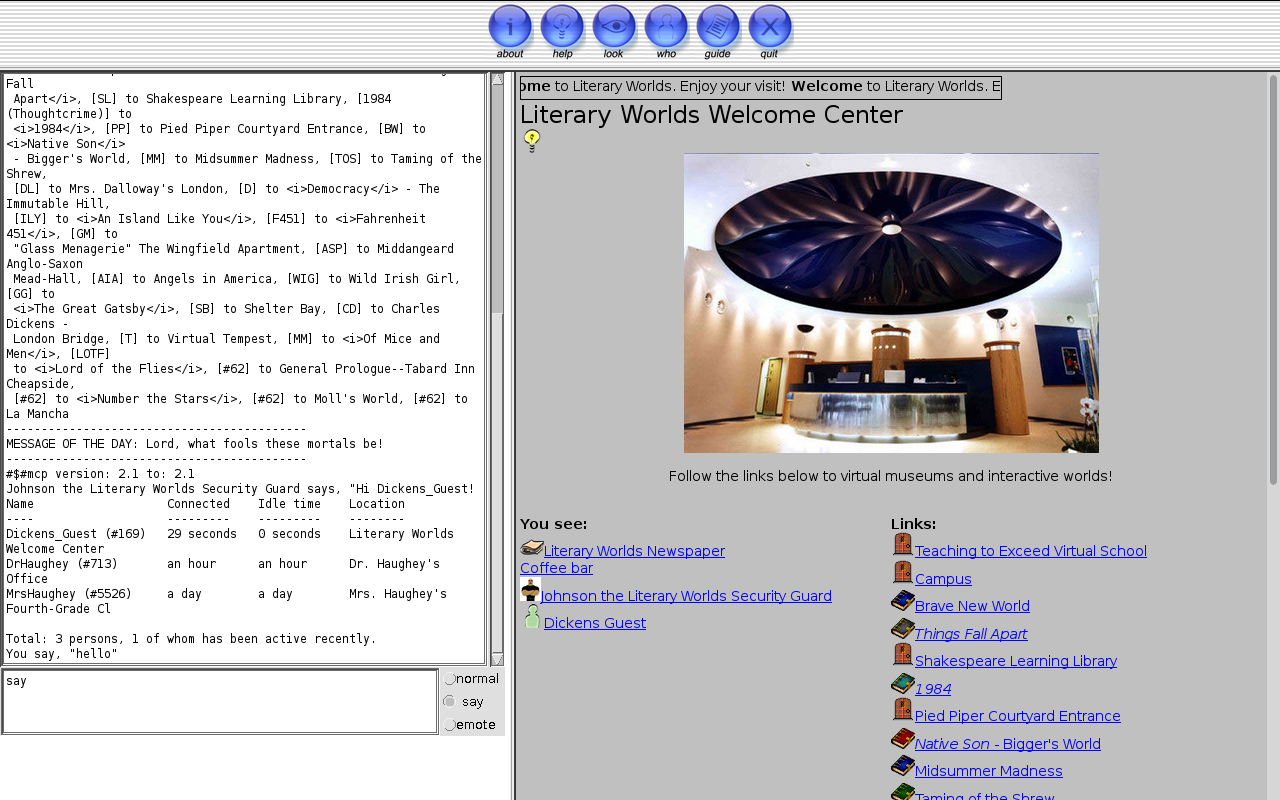
\includegraphics[width=\textwidth,height=\textheight,keepaspectratio]{classUsage.png}
\end{centering}
}

\section{Design Decisions}
\frame{\frametitle{Client-Server Design}
It is not possible to initiate a raw TCP connection in clientside Javascript, unlike Java applets.\\
Therefore, we need an intermediary server to connect over TCP, as well as to the browser client, and send data back and forth between the two.\\
This server must also support multiple concurrent users and handle asynchronous tasks and events.
}

\frame{\frametitle{Client-Server Diagram}
}

\frame{\frametitle{Client Technology}
% Backbone, Bootstrap, Socket.io, Coffeescript
\begin{itemize}
\item Socket.io
  \begin{itemize}
    \item Allows realtime communication between a server program and browser clients.
  \end{itemize}
  
\item Backbone
  \begin{itemize}
    \item Backbone is a templating library for Javascript web applications
  \end{itemize}
  
\item Bootstrap
  \begin{itemize}
	\item Bootstrap is a frontend layout toolkit
  \end{itemize}
  
\item Coffeescript
  \begin{itemize}
    \item Coffeescript is a whitespace language that translates to Javascript
    
  \end{itemize}
\end{itemize}
}

\frame{\frametitle{Server Technology}
% Node.JS here
\begin{itemize}
\item Node.js 
  \begin{itemize}
  \item It is the first class citizen for socket.io, so it was natural to choose it for the server.
  \item Node.js is a server side runtime that exploits the asynchronous features of Javascript to build asynchronous server side programs. It provides a rich set of networking libraries, and uses the Google Chrome Javascript engine, V8.
  \end{itemize}
\item Express
  \begin{itemize}
  \item Express is a web app framework for Node.js
  
  \end{itemize}
\end{itemize}
}


\section{Stories}
\frame{\frametitle{Stories}

}

\section{Implementation}
\frame{\frametitle{Continuous Integration}

}

\frame{\frametitle{Unit Testing}
}

\frame{\frametitle{Stories}

}

\section{Stories}
\frame{\frametitle{Stories}

}
\end{document}
